\documentclass[tikz,border=2pt]{standalone}
\usepackage{amsmath}
\usetikzlibrary{arrows.meta}
\begin{document}
% Left: the entry game tree (perfect information): root x_0 where E moves, decision node of I,
% terminal nodes with payoffs (v_E, v_I) = (0,2), (1,1), (-1,-1).
% Right: player 2 does not observe player 1's choice (O or F), so her two nodes form one
% information set (dashed): imperfect information, the simultaneous Battle of the Sexes.
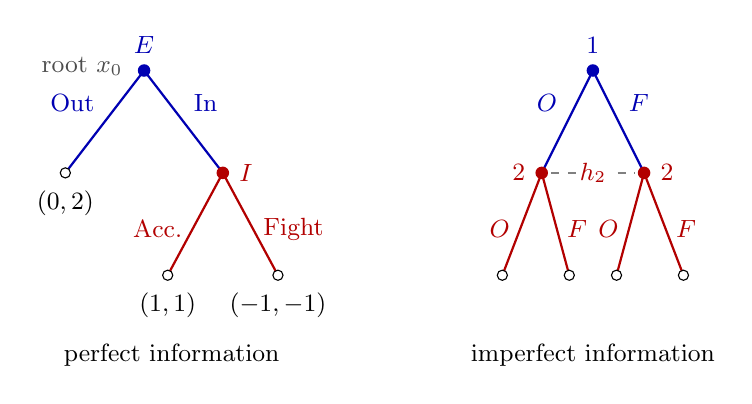
\begin{tikzpicture}[font=\small, >={Latex[length=2mm]},
    dec/.style={circle, fill, inner sep=1.6pt},
    term/.style={circle, draw, fill=white, inner sep=1.3pt}]
  % ---------- left: entry game ----------
  \draw[thick, blue!70!black] (1.0,0) -- node[above left, pos=0.5] {Out} (0,-1.3);
  \draw[thick, blue!70!black] (1.0,0) -- node[above right, pos=0.5] {In} (2.0,-1.3);
  \draw[thick, red!70!black] (2.0,-1.3) -- node[left, pos=0.55] {Acc.} (1.3,-2.6);
  \draw[thick, red!70!black] (2.0,-1.3) -- node[right, pos=0.55] {Fight} (2.7,-2.6);
  \node[dec, blue!70!black, label={[blue!70!black]above:$E$}] at (1.0,0) {};
  \node[dec, red!70!black, label={[red!70!black]right:$I$}] at (2.0,-1.3) {};
  \node[term] at (0,-1.3) {};
  \node[term] at (1.3,-2.6) {};
  \node[term] at (2.7,-2.6) {};
  \node[anchor=north] at (0,-1.4) {$(0,2)$};
  \node[anchor=north] at (1.3,-2.7) {$(1,1)$};
  \node[anchor=north] at (2.7,-2.7) {$(-1,-1)$};
  \node[gray!60!black, anchor=east] at (0.85,0.05) {root $x_0$};
  \node[anchor=north] at (1.35,-3.35) {perfect information};
  % ---------- right: one information set ----------
  \begin{scope}[xshift=5.4cm]
    \draw[thick, blue!70!black] (1.3,0) -- node[above left, pos=0.5] {$O$} (0.65,-1.3);
    \draw[thick, blue!70!black] (1.3,0) -- node[above right, pos=0.5] {$F$} (1.95,-1.3);
    \draw[thick, red!70!black] (0.65,-1.3) -- node[left, pos=0.55] {$O$} (0.15,-2.6);
    \draw[thick, red!70!black] (0.65,-1.3) -- node[right, pos=0.55] {$F$} (1.0,-2.6);
    \draw[thick, red!70!black] (1.95,-1.3) -- node[left, pos=0.55] {$O$} (1.6,-2.6);
    \draw[thick, red!70!black] (1.95,-1.3) -- node[right, pos=0.55] {$F$} (2.45,-2.6);
    \draw[dashed, thick, gray] (0.77,-1.3) -- (1.83,-1.3);
    \node[dec, blue!70!black, label={[blue!70!black]above:$1$}] at (1.3,0) {};
    \node[dec, red!70!black, label={[red!70!black]left:$2$}] at (0.65,-1.3) {};
    \node[dec, red!70!black, label={[red!70!black]right:$2$}] at (1.95,-1.3) {};
    \foreach \x in {0.15,1.0,1.6,2.45} \node[term] at (\x,-2.6) {};
    \node[red!70!black, fill=white, inner sep=1pt] at (1.3,-1.3) {$h_2$};
    \node[anchor=north] at (1.3,-3.35) {imperfect information};
  \end{scope}
\end{tikzpicture}
\end{document}
